\section*{Task Allocation}

\vspace{-0.5cm}

\section*{Definition}

\textbf{Task Allocation} is the problem of deciding "who does what, where, when and how" in a multi-robot system.

It involves finding a mapping / allocation A: T → R, which assigns a set of $n_t$ tasks (T) to a set of $n_r$ robots (R).

The goal is to find an assignment that maximizes overall global system utility.

\textbf{Division of labor} = the pattern or state resulting from that process (how work is distributed)

Tasl allocation can be:
\begin{itemize}
    \item Explicit: a central controller explicitly assigns task 1 to robot A, etc 
    \item Emergent: a division of labor emerges from local interactions, without any central controller
\end{itemize}

\section*{Formal Definition of MRTA}

We are given:
\begin{itemize}
    \item Set of robots, $R$
    \item Set of tasks, $T$
    \item $\mathtt{R} = 2^R$ set of all possible robot subteams
    \item A utility function:
    \[U_{rt} = Q_{rt} - C_{rt}\] for example, where $Q$ is quality and $C$ is cost
\end{itemize}

We need to find an allocation $A$ (mapping from tasks to robots) that maximizes 
global objective $U(A)$

\section*{MRTA Taxonomy}

\begin{table}[h!]
\centering
\renewcommand{\arraystretch}{1.2}
\begin{tabularx}{\textwidth}{@{}>{\centering\arraybackslash}p{3cm}|
                                  >{\centering\arraybackslash}p{2.5cm}|
                                  >{\centering\arraybackslash}p{2.5cm}|
                                  X@{}}
\toprule
\textbf{Dimension} & \textbf{Type 1} & \textbf{Type 2} & \textbf{Description} \\ \midrule
Robot Tasking (R) & Single-Task (ST) & Multi-Task (MT) & Can a single robot work on one task (ST) or multiple tasks simultaneously (MT)? \\ \addlinespace
Task Type (T) & Single-Robot (SR) & Multi-Robot (MR) & Does a task require one robot (SR) or a coalition/team of robots (MR)? \\ \addlinespace
Assignment Time (A) & Instantaneous Assignment (IA) & Time-Extended Allocation (TA) & Is the assignment instantaneous or one-shot (IA), or does it involve planning a schedule or route over time (TA)? \\
\bottomrule
\end{tabularx}
\caption{Dimensions of multi-robot task allocation (MRTA) taxonomy.}
\label{tab:mrta-dimensions}
\end{table}

\section*{Optimization Models for MRTA Problems}

\subsection*{The "Hello World": ST-SR-IA}
The simplest MRTA problem is the ST-SR-IA problem, where each robot can only do one task at a time (ST), each task requires only one robot (SR), and the assignment is instantaneous (IA).

Linear Assignment Problem (LAP) Solution: The optimal assignment can be found in polynomial time using the Hungarian Algorithm with a complexity of O($n^3$), (where n is the number of robots/tasks).

\begin{table}[h!]
\centering
\renewcommand{\arraystretch}{1.2}
\begin{tabularx}{\textwidth}{@{}p{2.5cm}|p{6.7cm}|X@{}}
\toprule
\textbf{Scenarios} & \textbf{Quick Definition} & \textbf{Important Result / Insight} \\ \midrule
\textbf{Adding Task Priorities} & Tasks have priority weights \(w_t\) indicating importance, added to the objective function. & Weighted assignment maximizes total utility \(\sum_r \sum_t w_t U_{rt} x_{rt}\). \\ \addlinespace
\textbf{$|R| \neq |T|$ (Unequal sets)} & Number of robots and tasks differ. Use dummy robots/tasks to balance. & Two IA rounds preserve polynomial-time solvability without affecting optimal real assignments. \\ \addlinespace
\textbf{Iterated Assignment} & Utilities or task info change over time → recompute or adaptively update assignments. & BLE (2001): 2-competitive ($\geq$50\% of optimal); L-ALLIANCE (1998): learns best assignments iteratively. \\ \addlinespace
\textbf{Online Assignment} & Tasks revealed one-by-one; robots may not be reassignable. & MURDOCH (2002): greedy, 3-competitive; best possible for online assignment without reassignment. \\
\bottomrule
\end{tabularx}
\label{tab:st-sr-ia-summary}
\end{table}

\subsection*{Other MRTA Scenarios}
\begin{itemize}
    \item \textbf{ST–SR–TA:} Find disjoint routes or schedules for multiple robots to visit all tasks, minimizing total travel cost. \textit{Model/Complexity:} Multiple Traveling Salesperson Problem (mTSP), NP-Hard.

    \item \textbf{MT–SR–IA:} Assign multiple tasks to a single robot, constrained by robot capacity/resources, to maximize total utility. \textit{Model/Complexity:} Generalized Assignment Problem (GAP), NP-Hard.

    \item \textbf{MT–SR–TA: VRP:} Vehicle Routing Problem (VRP). Find optimal routes for a fleet of vehicles to serve a set of customers/tasks, including constraints like limited capacity and time windows. \textit{Model/Complexity:} VRP, NP-Hard.

    \item \textbf{ST–SR–TA + Dependencies:} ST–SR–TA with precedence constraints (e.g., Task A must be completed before Task B can begin). \textit{Model/Complexity:} Complex Scheduling / Precedence-Constrained Scheduling, NP-Hard.

    \item \textbf{Traveling Salesman Problem (TSP):} Find the shortest single tour that visits a set of \(n\) tasks (cities) exactly once and returns to the origin (single-robot route planning). \textit{Model/Complexity:} TSP, NP-Hard (\(O(2^n)\)).

    \item \textbf{Vehicle Routing Problems (General):} Generalization of mTSP, where vehicles must respect real-world constraints like capacity limits, time windows, and precedence. \textit{Model/Complexity:} VRP, NP-Hard.
\end{itemize}

\subsection*{Orienteering Problems (OP)}

Orienteering Problems involve selecting a subset of tasks/locations to visit while maximizing total collected scores/profit, subject to route and time constraints.

\begin{itemize}
    \item \textbf{Classic Orienteering Problem (Single Vehicle):} Also called Selective TSP, Maximum Collection, or Bank Robber Problem. Maximize profit collected within a route duration constraint.

    \item \textbf{Profitable Tour Problem:} Maximize profit minus travel cost for a single vehicle.

    \item \textbf{Prize Collecting Traveling Salesman Problem (PCTSP):} Minimize travel cost while achieving a given route profit, for a single vehicle.

    \item \textbf{Team Orienteering Problem (Multiple Vehicles):} Also called Multiple Tour Maximum Collection Problem. Maximize total profit across multiple vehicles under route duration constraints.
\end{itemize}

\subsection*{Set-Based Formulations}
\begin{itemize}
    \item \textbf{Set Covering:} Select a subset of activities so that all requirements are covered at least once, minimizing cost.
    → Models MT–MR–IA (robots may appear in multiple coalitions).
    \[
    \min \sum c_j x_j \quad s.t. \sum a_{ij} x_j \ge 1
    \]

    \item \textbf{Set Packing:} Select disjoint subsets to maximize profit — each task covered by \textit{at most one} robot.
    → Models ST–MR–IA (exclusive task allocation).
    \[
    \max \sum p_j x_j \quad s.t. \sum a_{ij} x_j \le 1
    \]

    \item \textbf{Set Partitioning:} All tasks covered \textit{exactly once} by disjoint subsets.
    → Base for routing/scheduling models (e.g., VRP).
    \[
    \sum a_{ij} x_j = 1
    \]
\end{itemize}

\subsection*{Set Models and Coalition Formation in MRTA}
\begin{itemize}
    \item \textbf{Set Covering:} All tasks covered, robots may overlap → models \textbf{MT–MR–IA}.
    \item \textbf{Set Packing:} Maximize unique task coverage (no overlap) → models \textbf{ST–MR–IA}.
    \item \textbf{Set Partitioning:} All tasks done once, strict non-overlap → used in routing/scheduling (\textbf{VRP, TSP}).
\end{itemize}

Task allocation often combines:
\begin{itemize}
    \item \textit{Selection} — choosing which agents or coalitions perform which tasks (set-based).
    \item \textit{Ordering} — sequencing or scheduling tasks for each agent (routing/scheduling).
\end{itemize}


\subsection*{SUMMARY, MAPPING MRTA TYPE TO OPTIMIZATION MODEL}

\begin{center}
    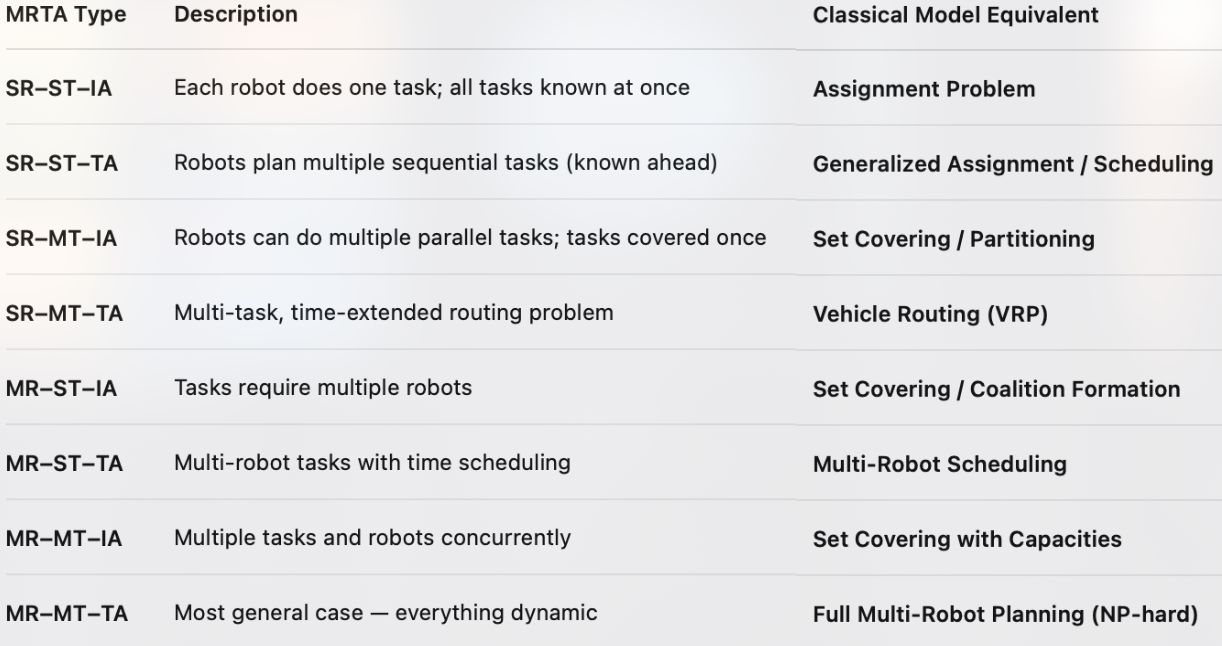
\includegraphics[width=0.8\textwidth]{../images/MRTA_Summary.png}
\end{center}
